\documentclass[english,onecolumn]{IEEEtran}
\usepackage[T1]{fontenc}
\usepackage[latin9]{luainputenc}
\usepackage[letterpaper]{geometry}
\geometry{verbose}
\usepackage{amsfonts}
\usepackage{babel}

\usepackage{extarrows}
\usepackage[colorlinks]{hyperref}
\usepackage{listings}
\usepackage{xcolor}
\usepackage[ruled,linesnumbered]{algorithm2e}

\usepackage{amsmath,graphicx}
\usepackage{subfigure} 
\usepackage{cite}
\usepackage{amsthm,amssymb,amsfonts}
\usepackage{textcomp}
\usepackage{bm}
\usepackage{booktabs}
\usepackage{listings}


\lstdefinestyle{mystyle}{
    numberstyle=\color{green},
    numbers=left,                    
    numbersep=5pt,                  
    showspaces=false,                
    showstringspaces=false,
    showtabs=false,                  
    tabsize=2
}

\lstset{style=mystyle}

\providecommand{\U}[1]{\protect\rule{.1in}{.1in}}
\topmargin            -18.0mm
\textheight           226.0mm
\oddsidemargin      -4.0mm
\textwidth            166.0mm
\def\baselinestretch{1.5}

\begin{document}

\begin{center}
	\textbf{{\Large SI231 - Matrix Computations, Fall 2020-21}}\\
	Homework Set \#2\\
   \texttt{Prof. Yue Qiu and Prof. Ziping Zhao} \\
	\texttt{\textbf{Name:}}   	\texttt{ Tian Yun }  		\hspace{1bp}
	\texttt{\textbf{Major:}}  	\texttt{ Master in CS } 	\\
	\texttt{\textbf{Student No.:}} 	\texttt{ 2019232102}     \hspace{1bp}
	\texttt{\textbf{E-mail:}} 	\texttt{ tianyun@shanghaitech.edu.cn}
\par\end{center}


\noindent
\rule{\linewidth}{0.4pt}
{\bf {\large Acknowledgements:}}
\begin{enumerate}
    \item Deadline: \textbf{2020-10-11 23:59:00}
    \item Submit your homework at \textbf{Gradescope}. Entry Code: \textbf{MY3XBJ}. Also, make sure that your gradescope account is your \textbf{school e-mail}.
    Homework \#2 contains two parts, the theoretical part the and the programming part.
    \item About the the theoretical part:
    \begin{enumerate}
            \item[(a)] Submit your homework in \textbf{Homework 2} in gradescope. Make sure that you have assigned the correct pages for the problems in the outline.
            \item[(b)] Your homework should be uploaded in the \textbf{PDF} format, and the naming format of the file is not specified.
            \item[(c)] No handwritten homework is accepted. You need to use \LaTeX. (If you have difficulty in using \LaTeX, you are allowed to use \textbf{Word} for the first and the second homework to accommodate yourself.)
            \item[(d)] Use the given template and give your solution in English. Solution in Chinese is not allowed. 
        \end{enumerate}
  \item About the programming part:
  \begin{enumerate}
      \item[(a)] Submit your codes in \textbf{Homework 2 Programming part} in gradescope.
      \item[(b)] Details of requirements in programming are listed in remarks of Problem 6, please read it carefully before you start to program.
  \end{enumerate}
  \item \textbf{No late submission is allowed.}
\end{enumerate}
\rule{\linewidth}{0.4pt}
\newpage 
\section{General Linear System}
\noindent\textbf{Problem 1}   \textcolor{blue}{(6 points + 9 points)}
\vspace*{3mm}

\noindent Let $\mathbf{A} = \begin{bmatrix}
	1 & 0 & 1 & 2\\
	-2 & 4 & -6 & 0\\
	3 & 1 & 14 & -1\\
	-1 & 7 & -5 & 3
	\end{bmatrix} \in\mathbb{R}^{4\times 4}\;$ and
	$\mathbf{B} = \begin{bmatrix}
	1 & 2 & 3 & -1\\
	2 & 3 & 1 & 1\\
	2 & 2 & 2 & -1\\
	5 & 5 & 2 & 3
	\end{bmatrix} \in\mathbb{R}^{4\times 4}\;.$
\begin{enumerate}
	\item 
	For {\bf A} and ${\bf b} = (-1,2,5,3)^T\in \mathbb{R}^4$, 
	find $\mathcal{N}({\bf A}),\, \mathcal{R}({\bf A})$, then solve ${\bf Ax} = {\bf b}$.
	\item 
	For {\bf B} and 
	${\bf b} = (1,1,1,2)^T \in \mathbb{R}^4$, solve the linear equation system ${\bf Bx} = {\bf b}$ 
	with Gauss Elimination, LU decomposition, and LU decomposition with partial pivoting, respectively. (Although not required, you are highly encouraged to write down your solution procedures in detail.)
\end{enumerate}

\noindent\textbf{Solution.}
\begin{enumerate}
    \item Nullspace is the space of all solutions  of $\mathbf{A}x$ = 0.
    
    $\mathbf{A}x = 
    \left[\begin{array}{cccc}
    	1 & 0 & 1 & 2\\
    	-2 & 4 & -6 & 0\\
    	3 & 1 & 14 & -1\\
    	-1 & 7 & -5 &3 
    \end{array}\right]
	\left[\begin{array}{c}
		x_1\\
		x_2\\
		x_3\\
		x_4 
	\end{array}\right]=0
$ 

After simplification:

    $[\mathbf{A| 0}] = 
\left[\begin{array}{cccc|c}
	1 & 0 & 0 & \frac{8}{3} &0\\
	0 & 1 & 0 & \frac{1}{3} &0\\
	0 & 0 & 1 & -\frac{2}{3} &0\\
	0 & 0 & 0 & 0 &0
\end{array}\right]
$

    $\mathbf{A}x = 
\left[\begin{array}{cccc}
	1 & 0 & 0 & \frac{8}{3}\\
	0 & 1 & 0 & \frac{1}{3}\\
	0 & 0 & 1 & -\frac{2}{3}\\
	0 & 0 & 0 & 0
\end{array}\right]
\left[\begin{array}{c}
	-\frac{3}{8}\\
	-\frac{1}{3}\\
	\frac{2}{3}\\
	1 
\end{array}\right]=0
$ 

$
	N(A)=\operatorname{span}\left(\left[\begin{array}{c}
	-\frac{3}{8}\\
-\frac{1}{3}\\
\frac{2}{3}\\
1 
	\end{array}\right]\right)
$

Then the column space of A is the space formed by all column vectors in A. The column space of A is represented by C(A)

$\mathbf{A}x = 
\left[\begin{array}{llll}
    	1 & 0 & 1 & 2\\
	-2 & 4 & -6 & 0\\
    	3 & 1 & 14 & -1\\
	 -1 & 7 & -5 &3 
\end{array}\right]
\left[\begin{array}{c}
x_1\\
x_2\\
x_3\\
x_4 
\end{array}\right]=
x_1\left[\begin{array}{c}
	1\\
	-2\\
	3\\
	-1 
\end{array}\right]=
x_2\left[\begin{array}{c}
	0\\
	4\\
	1\\
	7 
\end{array}\right]+
x_3\left[\begin{array}{c}
	1\\
	-6\\
	14\\
	-5 
\end{array}\right]+
x_4\left[\begin{array}{c}
	2\\
	0\\
	-1\\
	3 
\end{array}\right]
$

$
\mathcal{R}(A)=\operatorname{span}\left(\left[\begin{array}{l}
	1\\
-2\\
3\\
-1 
\end{array}\right]\left[\begin{array}{l}
	0\\
4\\
1\\
7 
\end{array}\right]\left[\begin{array}{l}
	1\\
-6\\
14\\
-5 
\end{array}\right]\left[\begin{array}{l}
	2\\
0\\
-1\\
3 
\end{array}\right]\right)=
\operatorname{span}\left(\left[\begin{array}{l}
	1\\
0\\
0\\
\frac{13}{8}
\end{array}\right]\left[\begin{array}{l}
	0\\
1\\
0\\
\frac{12}{16} 
\end{array}\right]\left[\begin{array}{l}
0\\
0\\
1\\
\frac{1}{4}
\end{array}\right]\right)
$

$A \vec{x}=\vec{b}$ When is there a solution?

The following two propositions are equivalent

1. When $\vec{b} \in C(A)$ , $\quad A \vec{x}=\vec{b}$ there a solution

2. When ${\operatorname{rank}}(A)=\operatorname{rank}(A, \vec{b})$ , $\quad A \vec{x}=\vec{b}$ there a solution

The general solution of the system of non-homogeneous linear equations $Ax=b$ is the general solution of the system of homogeneous linear equations$Ax=b$, plus any special solution of the system of non-homogeneous linear equations $Ax=b$:

So the solution of $Ax=b$:

$$
x = C \left[\begin{array}{c}
	-\frac{3}{8}\\
	-\frac{1}{3}\\
	\frac{2}{3}\\
	1 
\end{array}\right] + 
\left[\begin{array}{c}
	-\frac{5}{3}\\
	\frac{2}{3}\\
	\frac{2}{3}\\
	1 
\end{array}\right] 
$$

    \item 
    
    \begin{enumerate}
    	
		 	
		\item gauss decomposition
		
		$[\mathbf{B}|b] = \left[\begin{array}{cccc|c}
		1 & 2 & 3 & -1&1\\
		2 & 3 & 1 & 1&1\\
		2 & 2 & 2 & -1&1\\
		5 & 5 & 2 & 3&2
		\end{array}\right] = 
		\left[\begin{array}{cccc|c}
			1 & 0 & 0 & 0 & \frac{1}{6}\\
			0 & 1 & 0  &0 & \frac{1}{6}\\
			0 & 0 & 1 & 0 &\frac{1}{6}\\
			0 & 0 & 0 & 0&0
		\end{array}\right]
		$    	
		
		 $
		 \left[\begin{array}{c}
		 	x_1\\
		 	x_2\\
		 	x_3\\
		 	x_4 
		 \end{array}\right] = \left[\begin{array}{c}
		 	\frac{1}{6}\\
		 	\frac{1}{6}\\
		 	\frac{1}{6}\\
		 	0
		 \end{array}\right]
		 $   	
		 
		 
		  \item LU decomposition
		  
		  $\mathbf{B}x = \begin{bmatrix}
		  	1 & 2 & 3 & -1\\
		  	2 & 3 & 1 & 1\\
		  	2 & 2 & 2 & -1\\
		  	5 & 5 & 2 & 3
		  \end{bmatrix}\left[\begin{array}{c}
		  	x_1\\
		  	x_2\\
		  	x_3\\
		  	x_4 
		  \end{array}\right] = 
		  \begin{bmatrix}
		  	1 & 0 & 0 & 0 \\
		  	2 & 1 & 0 & 0 \\
		  	2 & 2 & 1 & 0 \\
		  	5 & 5 & 2 & 1
		  \end{bmatrix}
		  \begin{bmatrix}
		  	1 & 2 & 3 & -1 \\
		  	0 & -1 & -5 & 3 \\
		  	0 & 0 & 6 & -5 \\
		  	0 & 0 & 0 & 3
		  \end{bmatrix}
		  \left[\begin{array}{c}
		  	x_1\\
		  	x_2\\
		  	x_3\\
		  	x_4 
		  \end{array}\right]
		  =
		  \left[\begin{array}{c}
		  	1\\
		  	1\\
		  	1\\
		  	2
		  \end{array}\right]
		  $
		  
		  Multiply the two matrices on the left to the right matrix
		  
		  $
		  \left[\begin{array}{c}
		  	x_1\\
		  	x_2\\
		  	x_3\\
		  	x_4 
		  \end{array}\right] = \left[\begin{array}{c}
		  	\frac{1}{6}\\
		  	\frac{1}{6}\\
		  	\frac{1}{6}\\
		  	0
		  \end{array}\right]
		  $
		  
		  \item LU decomposition with partial pivoting
		  
		  $\mathbf{P_1}\mathbf{B} = 
		  \begin{bmatrix}
		  	0 & 0 & 0 & 1\\
		  	0 & 1  & 0  & 0\\
		  	0 & 0 & 1 & 0\\
		  	1 & 0 & 0 & 0
		  \end{bmatrix}
	      \begin{bmatrix}
		  	1 & 2 & 3 & -1\\
		  	2 & 3 & 1 & 1\\
		  	2 & 2 & 2 & -1\\
		  	5 & 5 & 2 & 3
		  \end{bmatrix} = 
		  \begin{bmatrix}
		  	5 & 5 & 2 & 3\\
			2 & 3 & 1 & 1\\
			2 & 2 & 2 & -1\\
			1 & 2 & 3 & -1\\
		  \end{bmatrix}
	  $
	  
	  $
	  	\mathbf{B_2} = \mathbf{L_1P_1B_1}= 
	 	 \begin{bmatrix}
		  1 & 0 & 0 & 0\\
		  -0.4 & 1  & 0  & 0\\
		  -0.4 & 0 & 1& 0\\
		  -0.2 & 0 & 0 & 1
	 	 \end{bmatrix}
		\begin{bmatrix}
		  	5 & 5 & 2 & 3\\
			2 & 3 & 1 & 1\\
			2 & 2 & 2 & -1\\
			1 & 2 & 3 & -1\\
		\end{bmatrix}=
	 	 \begin{bmatrix}
		5 & 5 & 2 & 3\\
		0 & 1 & 0.2 & -0.2\\
		0 & 0 & 1.2 & -2.2\\
		0 & 1 & 2.6 & -1.6
		\end{bmatrix}	
		  $
		  
		  $\mathbf{P_2}\mathbf{B_2} = \mathbf{B_2}$
		  
	  $
		\mathbf{B_3} = \mathbf{L_2P_2B_2}= 
		\begin{bmatrix}
			1 & 0 & 0 & 0\\
			0 & 1  & 0  & 0\\
			0 & 0 & 1& 0\\
			0 & -1 & 0 & 1
		\end{bmatrix}
		\begin{bmatrix}
		5 & 5 & 2 & 3\\
		0 & 1 & 0.2 & -0.2\\
		0 & 0 & 1.2 & -2.2\\
		0 & 1 & 2.6 & -1.6
		\end{bmatrix}=
		\begin{bmatrix}
			5 & 5 & 2 & 3\\
			0 & 1 & 0.2 & -0.2\\
			0 & 0 & 1.2 & -2.2\\
			0 & 0 & 2.4 & -1.4
		\end{bmatrix}	
		$
		  
		  $\mathbf{P_3}\mathbf{B_3} = 
		  	\begin{bmatrix}
		  	1 & 0 & 0 & 0\\
		  	0 & 1  & 0  & 0\\
		  	0 & 0 & 0& 1\\
		  	0 & 0 & 1& 0
		  \end{bmatrix}
		  \begin{bmatrix}
			5 & 5 & 2 & 3\\
			0 & 1 & 0.2 & -0.2\\
			0 & 0 & 1.2 & -2.2\\
			0 & 0 & 2.4 & -1.4
		  \end{bmatrix}
		  $
		  
		  $
		  \mathbf{B_4} = \mathbf{L_3P_3B_3}= 
		  \begin{bmatrix}
		  	1 & 0 & 0 & 0\\
		  	0 & 1  & 0  & 0\\
		  	0 & 0 & 1& 0\\
		  	0 & 0 & -0.5 & 1
		  \end{bmatrix}
		  \begin{bmatrix}
		  	5 & 5 & 2 & 3\\
		  	0 & 1 & 0.2 & -0.2\\
		  	0 & 0 & 2.4 & -1.4\\
		  	0 & 0 & 1.2 & -2.2
		  \end{bmatrix}	=
	  	\begin{bmatrix}
		  5 & 5 & 2 & 3\\
		  0 & 1 & 0.2 & -0.2\\
		  0 & 0 & 2.4 & -1.4\\
		  0 & 0 & 0 & -1.5
	  	\end{bmatrix}
		  $
		  
		  Therefore, $P B=L U$ where
		  $$
		  L=L_{1}^{\prime-1} L_{2}^{\prime-1}L_{3}^{\prime-1}
		  $$
		  with $L_{3}^{\prime}= L_{3} ,$ $L_{2}^{\prime}=P_{3} L_{2} P_{3}^{-1},$ and $L_{1}^{\prime}=P_{3} P_{2}L_{1}P_2^{-1} P_{3}^{-1},$
		  $$
		  U=\begin{bmatrix}
		  	5 & 5 & 2 & 3\\
		  	0 & 1 & 0.2 & -0.2\\
		  	0 & 0 & 2.4 & -1.4\\
		  	0 & 0 & 0 & -1.5
		  \end{bmatrix}
		  $$
		  and
		  $$
		  P=P_{3}P_{2} P_{1}
		  $$
		  In general, for an $n \times n$ matrix $A,$ the LU factorization provided by Gaussian elimination
		  with partial pivoting can be written in the form:
		  $$
		  \left(L_{n-1}^{\prime} \cdots L_{2}^{\prime} L_{1}^{\prime}\right)\left(P_{n-1} \cdots P_{2} P_{1}\right) A=U
		  $$
		  where $L_{i}^{\prime}=P_{n-1} \cdots P_{i+1} L_{i} P_{i+1}^{-1} \cdots P_{n-1}^{-1}$
		  If $L=\left(L_{n-1}^{\prime} \cdots L_{2}^{\prime} L_{1}^{\prime}\right)^{-1}$ and $P=P_{n-1} \cdots P_{2} P_{1},$ then $P A=L U$
		  
		  $
		  PB = LU, B = p^{-1}LU, Bx = b,p^{-1}LUx = b, x = U^{-1}L^{-1}Pb
		  $
		  
		  $
		  \left[\begin{array}{c}
		  	x_1\\
		  	x_2\\
		  	x_3\\
		  	x_4 
		  \end{array}\right] = \left[\begin{array}{c}
		  	\frac{1}{6}\\
		  	\frac{1}{6}\\
		  	\frac{1}{6}\\
		  	0
		  \end{array}\right]
		  $
	 \end{enumerate}
	


\end{enumerate}


\newpage
\section{Understanding Various Matrix Decompositions}
\noindent\textbf{Problem 2} \textcolor{blue}{(10 points)}

\noindent Consider the following symmetric matrix ${\bf A}\in \mathbb{R}^{4\times 4}$,
	\begin{align*}
		\mathbf{A}=
		\begin{bmatrix}
			a&a&a&a\\
			a&b&b&b\\
			a&b&c&c\\
			a&b&c&d
		\end{bmatrix}\,.
	\end{align*}
Give the LU decomposition of $\mathbf{A}$.
Then describe under which conditions $\bf{A}$ is nonsingular, according to the results of LU decomposition.

\noindent \textbf{Solution.}

$\mathbf{A} = 
\begin{bmatrix}
	1 & 0 & 0 & 0\\
	1 & 1  & 0  & 0\\
	1 & 1 & 1& 0\\
	1 & 1 & 1& 1
\end{bmatrix}
\begin{bmatrix}
	a & a & a & a\\
	0 & -a+b & -a+b & -a+b\\
	0 & 0 & -b+c & -b+c\\
	0 & 0 & 0 & d-c
\end{bmatrix}
$

\par

First of all: a cannot be equal to 0. Under the premise that a is not equal to 0, b cannot be equal to a, and c cannot be equal to b, and d cannot be equal to c. So a is not equal to 0, then a, b, c, d are different from each other

\newpage
\noindent\textbf{Problem 3} \textcolor{blue}{(5 points + 10 points)}
\begin{enumerate}
	\item Consider a $3\times 3$ matrix
	\[
	\mathbf{A} = \begin{bmatrix}
		2& 2&4 \\
		1&5&1\\
		1&1&8
	\end{bmatrix}\,,
	\] find the LDM (also called LDU) decomposition of $\mathbf{A}$, i.e., factor $\mathbf{A}$ as $\mathbf{A}=\mathbf{L}\mathbf{D}\mathbf{M}^T$ (or $\mathbf{A}=\mathbf{L}\mathbf{D}\mathbf{U}$), where $\mathbf{L}\in\mathbb{R}^{3\times 3}$ is lower triangular with unit diagonal entries, $\mathbf{D}\in\mathbb{R}^{3\times 3}$  is  a diagonal matrix, and $\mathbf{M}\in\mathbb{R}^{3\times 3}$ is lower triangular with unit diagonal entries ($\mathbf{U}\in\mathbb{R}^{3\times 3}$ is upper triangular with unit diagonal entries).
	
	\item Consider a $3\times 3$ matrix
	\[
	\mathbf{B} = \begin{bmatrix}
		8& 1&1 \\
		1&5&1\\
		4&2&2
	\end{bmatrix}\,,
	\] find the UL decomposition  of $\mathbf{B}$, 
	i.e., factor $\mathbf{B}$ as $\mathbf{B} = \mathbf{UL}$,
	where $\mathbf{U}\in\mathbb{R}^{3\times 3}$ is upper triangular with unit diagonal entries and $\mathbf{L}\in\mathbb{R}^{3\times 3}$ is lower triangular.\\
	\textbf{Hint:}  $\mathbf{B}=\mathbf{P}\mathbf{A}\mathbf{P}$, where $\mathbf{P}$ is a unit anti-diagonal matrix \footnote{{\textbf{Anti-diagonal matrix:} An anti-diagonal matrix is a square matrix where all the entries are zero except those on the diagonal going from the lower left corner to the upper right corner, known as the anti-diagonal. For example, 
			\[
			\text{adiag}(a_1,\ldots,a_n) = \begin{bmatrix}
				0 & 0 & \cdots & 0 & a_1 \\
				0 & 0 & \cdots  & a_2 & 0 \\
				\vdots &  \vdots & \ddots & \vdots &\vdots \\
				a_n & 0 & \cdots &  \cdots& 0
			\end{bmatrix}\,,
			\]
			and consequently, unit anti-diagonal matrix means $\text{adiag}(1,\ldots,1)$, also known as the \textbf{exchange matrix} or the \textbf{permutation matrix}. 
	}}.
\end{enumerate}
\noindent\textbf{Solution.}
\begin{enumerate}
    \item 
    
    	$
    \mathbf{A} = \mathbf{LU}=
    \begin{bmatrix}
    	2& 2&4 \\
    	1&5&1\\
    	1&1&8
    \end{bmatrix}=
    \begin{bmatrix}
	8& 1&1 \\
	1&5&1\\
	4&2&2
\end{bmatrix}=
\begin{bmatrix}
	1& 0&0 \\
	\frac{1}{2}&1&0\\
	\frac{1}{2}& 0 &1
\end{bmatrix}\
\begin{bmatrix}
	2& 2&4 \\
	0&4&-1\\
	0&0&6
\end{bmatrix}
=\mathbf{LDU}=
    \begin{bmatrix}
	1& 0&0 \\
	\frac{1}{2}&1&0\\
	\frac{1}{2}& 0 &1
	\end{bmatrix}\
	\begin{bmatrix}
		2& 0&0 \\
		0&4&0\\
		0&0&6
	\end{bmatrix}
	\begin{bmatrix}
	1& 1&2 \\
	0&1&-\frac{1}{4}\\
	0&0&1
	\end{bmatrix}
   $
    
    \item 
    
    $
    \mathbf{B} =\mathbf{PAP} 
    =\mathbf{PLUP}= \mathbf{(PLP^T)(PUP^T)}=
    \begin{bmatrix}
    	8& 1&1 \\
    	1&5&1\\
    	4&2&2
    \end{bmatrix}=
    \begin{bmatrix}
	1& 0&0 \\
	\frac{1}{2}&1&0\\
	\frac{1}{2}& 0 &1
    \end{bmatrix}\
    \begin{bmatrix}
	2& 2&4 \\
	0&4&-1\\
	0&0&6
    \end{bmatrix}
    $
    
    $
    \mathbf{B} =
    \begin{bmatrix}
	0& 0&1 \\
	0&1&0\\
	1& 0 &0
	\end{bmatrix}
    \begin{bmatrix}
    	1& 0&0 \\
    	\frac{1}{2}&1&0\\
    	\frac{1}{2}& 0 &1
    \end{bmatrix}
    \begin{bmatrix}
	0& 0&1 \\
	0&1&0\\
	1& 0 &0
\end{bmatrix}
    \begin{bmatrix}
	0& 0&1 \\
	0&1&0\\
	1& 0 &0
\end{bmatrix}
    \begin{bmatrix}
    	2& 2&4 \\
    	0&4&-1\\
    	0&0&6
    \end{bmatrix}
    \begin{bmatrix}
	0& 0&1 \\
	0&1&0\\
	1& 0 &0
\end{bmatrix}
    $
    
    
    Let $B=P A P$ where $P$ is the permutation matrix with 1 's on the anti-diagonal and 0's elsewhere. Thus $P=P^{T}=P^{-1},$ and $B$ is orthogonally similar to $A$
    
    If $A=L U$ is a factorization with lower triangular $L$ having $1^{\prime}$ s along the diagonal, and $U$ an upper triangular matrix, then:
    $$
   B=\left(P L P^{T}\right)\left(P U P^{T}\right)
    $$
    Note that $P L P^{T}$ is an upper triangular matrix with 1 's along the diagonal, and $P U P^{T}$ is a lower triangular matrix, so the above is a factorization of the desired form.
    
    
       	$
    \mathbf{B} = 
    \left(P L P^{T}\right)\left(P U P^{T}\right)
    =
    \begin{bmatrix}
    	0& 0&1 \\
    	0&1&0\\
    	1& 0 &0
    \end{bmatrix}
    \begin{bmatrix}
    	1& 0&0 \\
    	\frac{1}{2}&1&0\\
    	\frac{1}{2}& 0 &1
    \end{bmatrix}
    \begin{bmatrix}
    	0& 0&1 \\
    	0&1&0\\
    	1& 0 &0
    \end{bmatrix}
    \begin{bmatrix}
    	0& 0&1 \\
    	0&1&0\\
    	1& 0 &0
    \end{bmatrix}
    \begin{bmatrix}
    	2& 2&4 \\
    	0&4&-1\\
    	0&0&6
    \end{bmatrix}
    \begin{bmatrix}
    	0& 0&1 \\
    	0&1&0\\
    	1& 0 &0
    \end{bmatrix}
    $ 
    
    $
    \mathbf{B} = 
    \left(P L P^{T}\right)\left(P U P^{T}\right)
    =
    \begin{bmatrix}
    	1& 0&\frac{1}{2} \\
    	0&1&\frac{1}{2}\\
    	0&0&1
    \end{bmatrix}
    \begin{bmatrix}
    	6& 0&0 \\
    	-1&4&0\\
    	4&2&2
    \end{bmatrix}
    $ 
    
\end{enumerate}

\newpage
\noindent\textbf{Problem 4} \textcolor{blue}{(7 points + 6 points + 7 points + 5 points)}

\noindent Given a matrix $\mathbf{A}\in\mathbb{R}^{n\times n}$, suppose that the LDM (LDU) decomposition of $\mathbf{A}$ exists, prove that
\begin{enumerate}
	\item the LDM (LDU) decomposition of $\mathbf{A}$ is \textit{uniquely} determined;
	\item if $\mathbf{A}$ is a symmetric matrix, then its LDM (LDU) decomposition must be $\mathbf{A}=\mathbf{L}\mathbf{D}\mathbf{L}^T$, which is called LDL (LDL$^T$) decomposition in this case;
	\item $\mathbf{A}$ is a symmetric and positive definite matrix if and only if its Cholesky decomposition exists (i.e., there exists a matrix $\mathbf{G}\in\mathbb{R}^{n\times n}$ such that $\mathbf{A}=\mathbf{G}\mathbf{G}^T$, where $\mathbf{G}$ is lower triangular with \textit{positive} diagonal entries);
	\item if $\mathbf{A}$ is a symmetric and positive definite matrix, then its Cholesky decomposition is \textit{uniquely} determined.	
\end{enumerate}

\textbf{Hints:}  
\begin{enumerate}
    \item The existence of the LDM (LDU) decomposition implies the non-singularity of the matrix.
    \item You can directly utilize the following lemmas,
\begin{itemize}
    \item the inverse (if it exists) of a lower (resp. upper) triangular matrix is also lower (resp. upper) triangular;
    \item the product of two lower (resp. upper) triangular matrices is lower (resp. upper) triangular;
    \item also, if such two lower (resp. upper) triangular matrices have unit diagonal entries, then their product also has unit diagonal entries.
\end{itemize}
\end{enumerate}

  

\noindent\textbf{Solution.}
\begin{enumerate}
    \item First of all, we want to prove that the LU decomposition is unique. 
    
    To prove LU is unique. Suppose that
    
    $$
    L_{1} U_{1}=L_{2} U_{2}
    $$
    
    where $L_{1}, L_{2}$ are unit lower triangular and $U_{1}, U_{2}$ are upper triangular and invertible. (They must be invertible if $L_{i} U_{i}$ is so.) We now rearrange the equation to get
    
    $$L_{2}^{-1} L_{1}=U_{2} U_{1}^{-1}$$
    
    Now the left side is unit lower triangular and the right side is upper triangular, but only the identity matrix satisies both conditions at once. Therefore we have
    
    $$L_{2}^{-1} L_{1}=I=U_{2} U_{1}^{-1}$$
    hence
    
    $$L_{1}=L_{2}, U_{1}=U_{2}$$
    
    proving the LU is uniqueness.
    
     If the LU decomposition is unique, then we change the upper and lower triangular matrices into triangular matrices with  diagonal elements are 1. because the integers are the same, then LDU is unique.
     
     \item Let $A$ be symmetric and $A=L D U^{\prime}$ be a LU-decomposition of $A$ where $D$ is a diagonal matrix and $u_{i, i}^{\prime}=1$
     $A=L D U^{\prime}=\left(L D U^{\prime}\right)^{T}=U^{T} D L^{T} . U^{T}$ is a lower left triangular matrix and $L^{T}$ is a upper right triangular matrix. This means $\left(L D U^{\prime}\right)^{T}$ is another LU-decomposition of $A$. But the decomposition is unique which implies $L=U^{\prime T}$ and $L^{T}=U^{\prime} .$ Hence $A=L D L^{T}$
     \item
    Suppose a matrix $A$ factors as $A=L^{*} L .$ Then
    $$
    \begin{aligned}
    	x^{*} A x &=x^{*} L^{*} L x \\
    	&=(L x)^{*}(L x) \\
    	&=\|L x\|^{2} \\
    	& \geq 0
    \end{aligned}
    $$
    This shows that $A$ is positive semidefinite.
    If we further assume that $L$ is square and triangular with positive real diagonal entries, then $L$ is invertible, so $L x=0 \Longleftrightarrow x=0 .$ In this case, we see that $A$ is positive definite.
     $$
     A=\mathbf{L}\mathbf{L}^*
     $$
    \item 
    The Cholesky decomposition of a positive-definite matrix A, is a decomposition of the form
    $$
    A=\mathbf{L}\mathbf{L}^*
    $$
    
	 Let $A$ be our positive definite matrix. Suppose $A$ has Cholesky factorizations $A=R^{*} R=S^{*} S$, for $R, S$ upper-triangular matrices with positive diagonal entries. Then we can write
	$$
	\langle A x, x\rangle=\langle R x, R x\rangle=\langle S x, S x\rangle
	$$
	Pick $x=e_{1},$ the first coordinate vector. Then $\langle A x, x\rangle=A_{11}=\left\|R e_{1}\right\|^{2}=\left\|S e_{1}\right\|^{2},$ and since $R, S$ are upper triangular, this uniquely defines the upper left entry of $R, S,$ so they must be the same. Now, the $k$ th entry in the first row of $R$ is given by
	$$
	\left\langle R e_{k}, e_{1}\right\rangle=\frac{1}{\sqrt{A_{11}}}\left\langle R e_{k}, R e_{1}\right\rangle=\frac{1}{\sqrt{A_{11}}}\left\langle A e_{k}, e_{1}\right\rangle
	$$
	so we in fact know the whole first row of $R$ and $S$, and they must be the same. Now, we reduce our $A$ to a new $(n-1) \times(n-1)$ submatrix, which will also be positive definite, and then repeat the procedure to uniquely determine the subsequent rows. 
	  
    
    
 
\end{enumerate}

\newpage
\noindent\textbf{Problem 5}
\textcolor{blue}{(10 points + 5 points)}

\noindent Consider matrix ${\bf A} \in \mathbb{R}^{n\times n}$ in the following form,
\[
\mathbf{A} = 
\begin{bmatrix}
	b_1 & c_1 &  0  &  0 & 0  & 0 \\
	a_2 & b_2 & c_2 &  0 & 0  & 0 \\
	0   & a_3 & b_3 & c_3 & 0 & 0 \\
	0   & 0 & \ddots & \ddots& \ddots&0\\
	\vdots & \vdots & \ddots& a_{n-1}& b_{n-1}& c_{n-1}\\
	0 & 0 & \cdots & 0 & a_{n} & b_n 
\end{bmatrix}\,,
\]
where $a_j$, $b_j$, and $c_j$ are non-zero entries.
The matrix in such form is known as a \textbf{Tridiagonal Matrix} in the sense that it contains three diagonals.
\begin{enumerate}
	\item LU decomposition is particularly efficient in the case of tridiagonal matrices. Find the LU decomposition of $\mathbf{A}$ (derivation is expected) and try to complete the Algorithm \ref{alg: lu_tri}.
\begin{algorithm}[htbp]
\SetKwInOut{Input}{Input}\SetKwInOut{Output}{Output}
\label{alg: lu_tri}
\caption{LU decomposition for tridiagonal matrices}
\SetAlgoLined
\Input{Tridiagonal matrix $\mathbf{A}\in \mathbb{R}^{n\times n}$.}
\Output{LU decomposition of $\mathbf{A}$.}

$v_{1}=b_1,$

For $k=2: n$

$\quad l_{k}=a_{k} / v_{k-1}$

$\quad$	Save $l_k$ in matrix L.

$\quad v_{k}=b_{k}-l_{k} e_{k-1}$

$\quad$	Save $v_k, c_k$ in matrix U.

End

Return L, U
\end{algorithm}



$$
\begin{aligned}
	&\left(\begin{array}{ccccc}
		b_{1} & c_{1} & & & \\
		a_{2} & b_{2} & c_{2} & & 0 \\
		& \ddots & \ddots & \ddots & \\
		& 0 & a_{n-1} & b_{n-1} & c_{n-1} \\
		& & & a_{n} & b_{n}
	\end{array}\right)=
	&\left(\begin{array}{ccccc}
		1 & & & &0 \\
		l_{2} & 1 & &  & \\
		& l_{3} & 1 & & \\
		& & \ddots & \ddots & \\
		0&  & &  l_{n} & 1
	\end{array}\right)\left(\begin{array}{ccccc}
		v_{1} & c_{1} & & &0 \\
		& v_{2} & c_{2} & &  \\
		& & \ddots & \ddots & \\
		& & & v_{n-1} & c_{n-1} \\
		0&  & & & v_{n}
	\end{array}\right)
\end{aligned}
$$
\item
Consider symmetric tridiagonal matrices
\[
\mathbf{A} = \begin{bmatrix}
    1 & 1 & 0\\
    1 & 2 & 1 \\
    0 & 1 & 2 
\end{bmatrix}
\quad \text{and  }
\mathbf{B}= \begin{bmatrix}
    a & a & 0 \\
    a & a+b & b \\
    0 & b & b+c
\end{bmatrix}\,,
\]
and give the LU decompositions and the LDL$^T$ (also known as the LDL) decompositions of $\mathbf{A}$ and $\mathbf{B}$ respectively.
\end{enumerate}
\noindent\textbf{Solution.}
\begin{enumerate}
    \item As shown above
    \item 
    $
    \mathbf{A} = \begin{bmatrix}
    	1 & 1 & 0\\
    	1 & 2 & 1 \\
    	0 & 1 & 2 
    \end{bmatrix}=LU=
	\begin{bmatrix}
		1 & 0 & 0\\
		1 & 1 & 0 \\
		0 & 1 & 1 
	\end{bmatrix}
	\begin{bmatrix}
	1 & 1 & 0\\
	0& 1 & 1\\
	0 & 0 & 1 
	\end{bmatrix}
    $
    
        $
    \mathbf{A} = \begin{bmatrix}
    	1 & 1 & 0\\
    	1 & 2 & 1 \\
    	0 & 1 & 2 
    \end{bmatrix}=LDL^T=
    \begin{bmatrix}
    	1 & 0 & 0\\
    	1 & 1 & 0 \\
    	0 & 1 & 1 
    \end{bmatrix}
    \begin{bmatrix}
	1 & 0& 0\\
	0& 1 & 0\\
	0 & 0 & 1 
	\end{bmatrix}
    \begin{bmatrix}
    	1 & 1 & 0\\
    	0& 1 & 1\\
    	0 & 0 & 1 
    \end{bmatrix}
    $
    
        $
    \mathbf{B} = \begin{bmatrix}
    	a & a & 0\\
    	a & a+b & b \\
    	0 & b & b+c 
    \end{bmatrix}=LU=
    \begin{bmatrix}
    	1 & 0 & 0\\
    	1 & 1 & 0 \\
    	0 & 1 & 1 
    \end{bmatrix}
    \begin{bmatrix}
    	a & a & 0\\
    	0& b & b\\
    	0 & 0 & c 
    \end{bmatrix}
    $
    
            $
    \mathbf{B} = \begin{bmatrix}
    	a & a & 0\\
    	a & a+b & b \\
    	0 & b & b+c 
    \end{bmatrix}=LU=
    \begin{bmatrix}
    	1 & 0 & 0\\
    	1 & 1 & 0 \\
    	0 & 1 & 1 
    \end{bmatrix}
    \begin{bmatrix}
	a & 0 & 0\\
	0 & b & 0 \\
	0 & 0 & c 
	\end{bmatrix}
    \begin{bmatrix}
    	1 & 1 & 0\\
    	0& 1 & 1\\
    	0 & 0 & 1 
    \end{bmatrix}
    $
\end{enumerate}

\newpage
\section{Programming}
\noindent\textbf{Problem 6}
\textcolor{blue}{(5 points + 15 points)}

\noindent In this problem, we explore  the efficiency of the LU method together with the classical linear system solvers we have learnt in linear algebra. 

\begin{enumerate}
	\item Derive the complexity of the LU decomposition. Particularly, how many flops does the LU decomposition require? The corresponding pseudo code (in {\sf Matlab}) is provided as follows: 
\begin{lstlisting}[language=Matlab]
function [L,U]= Naive_lu(A) 
    n = size(A,1)
    L = eye(n)
    U = A 
    for k=1:n-1
        for j=k+1:n
            L(j,k)=U(j,k)/U(k,k)
            U(j,k:n)=U(j,k:n)-L(j,k)*U(k,k:n)
        end
    end
    for k=2:n
        U(k,1:k-1)=0
    end
end
\end{lstlisting}
\item 
\textbf{Programming part:} 
Randomly generate a non-singular matrix $\mathbf{A}\in\mathbb{R}^{n\times n}$ and a vector $\mathbf{b}\in\mathbb{R}^{n\times 1}$, then program the following  methods to solve $\mathbf{Ax=b}$: 
\begin{itemize}
  \item {\bf The inverse method:} Use the inverse of $\mathbf{A}$ to solve the problem, which can be written as,
  \[
  \mathbf{x}=\mathbf{A}^{-1}\mathbf{b}\,.
  \]
  \item {\bf Cramer rule:} Suppose $\mathbf{x}=[x_1,\dots,x_n]^T$, and we denote $\mathbf{A}_{-i}(\mathbf{b})$ the matrix that we replace the $i$-th column of $\mathbf{A}$ with $\mathbf{b}$. Then we have
    \[
      x_i=\frac{\det(\mathbf{A}_{-i}(\mathbf{b}))}{\det(\mathbf{A})}, i=1,\dots,n\,.
    \]
  \item {\bf Gauss Elimination:} We perform row operations on the augmented matrix $[\mathbf{A}|\mathbf{b}]$, and use back substitution to obtain the solution $\mathbf{x}$.
  \item {\bf LU decomposition.} We first find the LU decomposition of $\mathbf{A}$, then we solve $\mathbf{L}\mathbf{y}=\mathbf{b}$ and $\mathbf{U}\mathbf{x}=\mathbf{y}$.
\end{itemize}
In your homework, you are required to submit the time-consuming plot (\textbf{one figure}) of given methods against the size of matrix $\mathbf{A}$ (i.e., $n$), where $n=100, 150,\dots, 1000$ (You can try larger $n$ and see what will happen, but be careful with the memory use of your PC!). 

\newpage

\noindent\textbf{Remarks: (Important!)}
\begin{itemize}
    \item Coding languages are restricted, but do not use any bulit-in function. For example, do not use {\sf Matlab} functions such as {\sf A/b}, {\sf inv(A)} or {\sf lu(A)}. Otherwise, your results will contradict the complexity analysis, and your scores will be discounted. You can implement the simplest version of these methods by yourself.
    \item When handing in your homework in gradescope, package all your codes into {\sf your\_student\_id+hw2\_code.zip} and upload. In the package, you also need to include a file named {\sf README.txt/md} to clearly identify the function of each file.
     \item Make sure that your codes can run and are consistent with your solutions.
  %\item In {\sf Matlab}, to randomly generate a matrix or a vector, you can use {\sf randn} function to generate normally distributed random numbers.
\end{itemize}
\end{enumerate} 

\noindent\textbf{Solution.}
\begin{enumerate}
    \item 
    
    1. For the first step $L(j,k)=U(j,k)/U(k,k)$ :
    $$\frac{[  (n-1)  + 1]  * (n-1)  }  {2  }    = \frac{n (n-1) }{ 2}$$
    
    2. For the  step $U(j,k:n)=U(j,k:n)-L(j,k)*U(k,k:n)$ :
    $$2[ (n-1)n + (n-2)(n-1)+...+2*1 ]   = \sum_1^n n^2 -n = 2 \frac{n(n+1)(2n+1)}{6}-2 \frac{(n+1)n}{2}$$
    
    3. For the  step $U(k,1:k-1)=0$ :
    $$\frac{[  (n-1)  + 1]  * (n-1)  }  {2  }    = \frac{n (n-1) }{ 2}$$
    
    $$SUM = \frac{n (n-1) }{ 2} + 2 \frac{n(n+1)(2n+1)}{6}-(n+1)n+ \frac{n (n-1) }{ 2} = \frac{2}{3}n^3+n^2-\frac{5}{3}n$$
    
    So the time complexity is $O(\frac{2}{3} n^3)$
    
    \item
    
    	\begin{figure}[h]
    	\centering
    	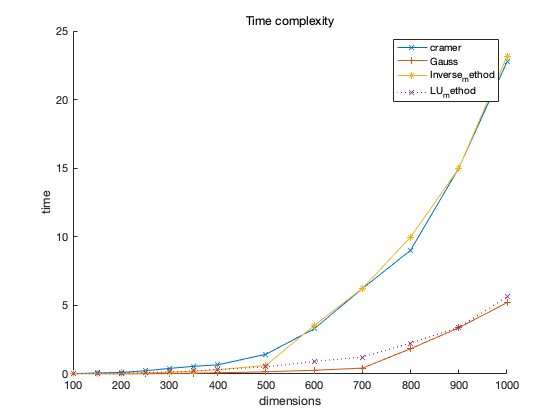
\includegraphics[width=0.8\textwidth]{Time_complexity.png}
  
    \end{figure}
    \begin{enumerate}
    
    \end{enumerate}
\end{enumerate}

\newpage

\section{Roundoff Error}
\noindent\textbf{Problem 7} \textcolor{blue}{(Bonus Problem: 10 points + 8 points + 2 points)}

Given a matrix $\mathbf{A}\in \mathbb{R}^{n\times n}$, consider the roundoff error in the process of solving $\mathbf{A}\bf{x} = \bf{b}$ by Gaussian elimination in three stages:
\begin{enumerate}
    \item[1.] Decompose $\mathbf{A}$ into $\mathbf{L}\mathbf{U}$, in a machine with roundoff error $\mathbf{E}$, $\bar{\mathbf{L}}$ and $\bar{\mathbf{U}}$ are computed instead, i.e., 
    \begin{equation*}
        \mathbf{A} + \mathbf{E} = \bar{\mathbf{L}}\bar{\mathbf{U}}\,.
    \end{equation*}
    \item[2.] Solving $\mathbf{L}\bf{y} = \bf{b}$, numerically with roundoff error $\delta \mathbf{\bar{L}}$, $\hat{\mathbf{y}} = \bf{y}+\delta \bf{y}$ are computed instead, i.e.,
    \begin{equation*}
        (\bar{\mathbf{L}}+\delta \bar{\mathbf{L}})(\bf{y}+\delta \bf{y}) = \bf{b}\,.
    \end{equation*}
    \item[3.] Solving $\mathbf{U}\bf{x} = \bf{y}$, numerically with roundoff error $\delta \mathbf{\bar{U}}$, $\hat{\bf{x}} = \bf{x}+\delta \bf{x}$ are computed instead, i.e.,
    \begin{equation*}
        (\bar{\mathbf{U}}+\delta \bar{\mathbf{U}})(\bf{x}+\delta \bf{x}) = \hat{y}\,.
    \end{equation*}
\end{enumerate}
Finally, we can get the computed solution $\hat{\bf{x}}$ and 
\begin{align*}
    \bf{b} = &(\bar{\mathbf{L}}+\delta \bar{\mathbf{L}})(\bar{\mathbf{U}}+\delta \bar{\mathbf{U}})(\bf{x}+\delta \bf{x})\\
     = & (\mathbf{A}+\delta \mathbf{A})(\bf{\bf{x}}+\delta \bf{\bf{x}})\,.
\end{align*}

\begin{enumerate}
    \item Prove that the relative error of $\bf{x}$ has an upper bound as follows,
    \begin{equation*}
        \frac{\|\hat{\mathbf{x}}-\mathbf{x}\|}{\|\mathbf{x}\|} = \frac{\|\delta \bf{x}\|}{\|\bf{x}\|} \leq \frac{1}{1-\kappa(\mathbf{A})\frac{\|\delta \mathbf{A}\|}{\|\mathbf{A}\|}}\kappa(\mathbf{A})\frac{\|\delta \mathbf{A}\|}{\|\mathbf{A}\|},
    \end{equation*}
    where $\kappa(\mathbf{A}) = \|\mathbf{A}\|\|\mathbf{A}^{-1}\|$ denotes the condition number of matrix $\mathbf{A}$ (Suppose $\mathbf{A}$ and $\mathbf{A}+\delta \mathbf{A}$ are nonsingular and $\|\mathbf{A}^{-1}\|\|\delta \mathbf{A}\|<1$), and $\|\cdot\|$ can be any norm.
    
    \textbf{Hint}: The following equation might be useful,
    \begin{align*}
        \|(\mathbf{I}-\mathbf{B})^{-1}\| =  \|\sum_{k = 0}^{\infty} \mathbf{B}^k\| \leq \sum_{k = 0}^{\infty} \|\mathbf{B}\|^k \leq  \frac{1}{1-\|\mathbf{B}\|}\,.
    \end{align*}
    
    % \begin{equation}
    %     (\mathbf{I}-\mathbf{A})^{-1} = \mathbf{I} + \mathbf{A} + \mathbf{A}^2 + ... = \sum_{k = 0}^\infty \mathbf{A}^{k},
    % \end{equation}
    
    where $\mathbf{I}-\mathbf{B}$ is nonsingular and $\lim_{n\to \infty}\mathbf{B}^n = \mathbf{0}$.
    
    \item Consider a linear system $\mathbf{A}\mathbf{x} = \mathbf{b}$, where
    
    \[
        \mathbf{A} = \begin{bmatrix}2 & -1 & 1 \\ -1 &10^{-10} &10^{-10}\\ 1 & 10^{-10} & 10^{-10}  \end{bmatrix},\quad \mathbf{b} = \begin{bmatrix}2(1+10^{-10}) \\ -10^{-10} \\10^{-10} \end{bmatrix}
    \]
    
    find the solution $\mathbf{x}$, and calculate the condition number of $\mathbf{A}$ with the matrix infinite norm\footnote{If $\mathbf{A}\in\mathbb{R}^{n\times n}$, then the matrix infinite norm is  $\|\mathbf{A}\|_{\infty} = \max_{1<i<n}\sum_{j = 1}^n|a_{i,j}|$.}, i.e. $\kappa_\infty(\mathbf{A}) = \|\mathbf{A}\|_\infty\|\mathbf{A}^{-1}\|_\infty$. Suppose $|\delta\mathbf{A}|<10^{-18}|\mathbf{A}|$\footnote{$|\mathbf{A}|\leq |\mathbf{B}|$ means each element in $\mathbf{A}$ is relative smaller to the corresponding element of $\mathbf{A}$}, use $\kappa_\infty(\mathbf{A})$ to verify that 
    \[
        \|\delta \mathbf{x}\|< 10^{-7} \|\mathbf{x}\|. 
    \]
    
    
    \item Discuss what you have observed from the previous 2 questions. What are the main factors that influence the relative error of the computed solution? Does the ill-conditioned matrix (i.e. the condition number is large) always lead to a large error of the solution?     
\end{enumerate}

\noindent\textbf{Solution.}
\begin{enumerate}
    \item
  Suppose the original equation has undergone some changes after being disturbed
    $$
    (A+\delta A)(x+\delta x)=b+\delta b
    $$
    Because $b=A x$ ,So we get:
    $$
    (A+\delta A) \delta x=\delta b-\delta A x
    $$
   Because $\left\|A^{-1}\right\|\|\delta A\|<1$
    $$
    \left\|\left(I+A^{-1} \delta A\right)^{-1}\right\| \leqslant \frac{1}{1-\left\|A^{-1}\right\|\|\delta A\|}
    $$
   $$A+\delta A=A\left(I+A^{-1} \delta A\right)$$
    $$
    \begin{aligned}
    	\delta x &=(A+\delta A)^{-1}(\delta b-\delta A x) \\
    	&=\left(I+A^{-1} \delta A\right)^{-1} A^{-1}(\delta b-\delta A x)
    \end{aligned}
    $$
    
    $$
    \|\delta x\| \leqslant\left\|\left(I+A^{-1} \delta A\right)^{-1}\right\|\left\|A^{-1}\right\|(\|\delta b\|+\|\delta A\|\|x\|)
    $$
    $$
    \leqslant \frac{\left\|A^{-1}\right\|}{1-\left\|A^{-1}\right\|\|\delta A\|}(\|\delta b\|+\|\delta A\|\|x\|)
    $$
     
    $$
    \frac{\|\delta x\|}{\|x\|} \leqslant \frac{\left\|A^{-1}\right\|\|A\|}{1-\left\|A^{-1}\right\|\|\delta A\|}\left(\frac{\|\delta A\|}{\|A\|}+\frac{\|\delta b\|}{\|b\|}\right)
    $$
   Because $\|b\| \leqslant\|A\|\|x\|$
    $$
     \frac{\|\hat{x}-x\|}{\|x\|} = \frac{\|\delta x\|}{\|x\|} \leq \frac{1}{1-\kappa(A)\frac{\|\delta A\|}{\|A\|}}\kappa(A)\frac{\|\delta A\|}{\|A\|},
     $$
    \item 
    $\kappa_\infty(\mathbf{A}) = \|\mathbf{A}\|_\infty\|\mathbf{A}^{-1}\|_\infty$ = $2*10^{10}$
    
        \begin{equation*}
    	\frac{\|\hat{\mathbf{x}}-\mathbf{x}\|}{\|\mathbf{x}\|} = \frac{\|\delta \bf{x}\|}{\|\bf{x}\|} \leq \frac{1}{1-\kappa(\mathbf{A})\frac{\|\delta \mathbf{A}\|}{\|\mathbf{A}\|}}\kappa(\mathbf{A})\frac{\|\delta \mathbf{A}\|}{\|\mathbf{A}\|},
    \end{equation*}

	$|\delta\mathbf{A}|<10^{-18}|\mathbf{A}|$
	
	$\frac{|\delta\mathbf{A}|}{|\mathbf{A}|}<10^{-18}$
	
	 \begin{equation*}
		\frac{\|\hat{\mathbf{x}}-\mathbf{x}\|}{\|\mathbf{x}\|} = \frac{\|\delta \bf{x}\|}{\|\bf{x}\|} \leq \frac{1}{1-10^{-18}*2*10^{10}}2*10^{10}*10^{-18}<10^{-7}
	\end{equation*}
    \item
\end{enumerate}

\end{document}
